%! TEX program = pdflatex

\documentclass[oneside,solution]{seu-ml-assign}

\title{Assignment}
\author{Xie xing}
\studentID{58122204}
\instructor{Xu-Ying Liu}
\date{\today}
\duedate{May 17, 2024}
\assignno{3}
\semester{SEU --- 2024 Spring}
\mainproblem{Support Vector Machine \& Bayesian Classifiers}

\begin{document}

\maketitle

% \startsolution[print]
%第一题SVM
\problem{Support Vector Machine }

%第一题第一问
\subsection{}


%第一题第一问(a)
\subsubsection{(a)}
Generalized Lagrangian function:
\begin{equation}\begin{aligned}       & L(\omega,b,\epsilon,\alpha,\mu)=\frac12||\omega||^2+C\sum_{i=1}^N\epsilon_i,-\sum_{i=1}^N
                     \alpha_i(y_i(\omega^Tx_i+b) -1 + \epsilon)-\sum_{i=1}^N\mu_i\epsilon_i\end{aligned}
\end{equation},
where $ \alpha_i >= 0, \mu_i >=0$.
% The dual problem is the minimax problem of the Lagrangian function, now we firstly calcuate the partial derivative of the Lagrangian function:
The dual problem of the original function is
\begin{equation}\max_{\alpha\geq0,\mu\geq0}\min_{\omega,b,\epsilon}L(\omega,b,\epsilon,\alpha,\mu)\end{equation}

Find the partial derivative :
\begin{equation}
  \nabla_{w}L(w,b,\epsilon,\alpha,\mu)=w-\sum_{i=1}^{N}\alpha_{i}y_{i}x_{i}=0
\end{equation}

\begin{equation}
  \nabla_{b}L(w,b,\epsilon,\alpha,\mu)=-\sum_{i=1}^{N}\alpha_{i}y_{i}=0
\end{equation}

\begin{equation}
  \nabla_{\epsilon_{i}}L(w,b,\epsilon,\alpha,\mu)=C-\alpha_{i}-\mu_{i}=0
\end{equation}

Solutions have to:
\begin{equation}\left.\left\{\begin{aligned}w                       & =\sum_{i=1}^N\alpha_iy_ix_i \\
               \sum_{i=1}^N\alpha_iy_i & =0                          \\
               C-\alpha_i-\mu_i        & =0\end{aligned}\right.\right.
\end{equation}

Bringing in $L(w,b,\epsilon,\alpha,\mu)$ gets:

\begin{equation}\min_{\omega,b,\epsilon}L(w,b,\epsilon,\alpha,\mu)=-\frac12\sum_{i=1}^N
  \sum_{j=1}^N\alpha_i\alpha_jy_iy_j\left(x_i\cdot x_j\right)+\sum_{i=1}^N\alpha_i
\end{equation}

calcuate the maximum of $\min_{\omega,b,\epsilon}L(w,b,\epsilon,\alpha,\mu)$ on $\alpha$, we get the dual problem:

\begin{equation}
  \max_{\alpha} -\frac{1}{2}\sum_{i}^{N}\sum_{j}^{N}\alpha_i\alpha_jy_iy_j(x_i \cdot x_j)+\sum_{i=1}^{N}\alpha_{i}
\end{equation}

\begin{equation}
  s.t.\sum_{i}^{N}\alpha_iy_i=0
\end{equation}

\begin{equation}
  C-\alpha_i-\mu_i=0
\end{equation}

\begin{equation}
  \alpha_i \geq 0
\end{equation}

\begin{equation}
  \mu_i \geq 0, i = 1,2,...,N
\end{equation}


% Next, we originally found the maximum value of the above equation.
% If we add a negative sign to the entire equation, we can transform it into finding its minimum value, that is,
% \begin{equation}\min_\alpha\frac12\sum_{i=1}^N\sum_{j=1}^N\alpha_i\alpha_ju_iy_j\left(x_i\right.\cdot x_j)-\sum_{i=1}^N\alpha \end{equation}

% After getting the objective function, sort out the constraints.
First of all, there is a partial derivative solution $\sum_{i=1}^N\alpha_iy_i=0$,;\\
Secondly, the Lagrange multiplier is greater than or equal to 0, that is $\alpha, \mu >=0$,
when seeking partial derivatives, we get $C-\alpha_i-\mu_i=0$;\\
Finally, comprehensively we get $0\leq\alpha_i\leq C$.

So the dual problem is:

\begin{equation}
  \max_{\alpha} -\frac{1}{2}\sum_{i}^{N}\sum_{j}^{N}\alpha_i\alpha_jy_iy_j(x_i \cdot x_j)+\sum_{i=1}^{N}\alpha_{i}
\end{equation}

\begin{equation}
  s.t.\sum_{i}^{N}\alpha_iy_i=0
\end{equation}

\begin{equation}
  0\leq \alpha_i \leq C
\end{equation}




%第一题第一问(b)
\subsubsection{(b)}
At the saddle point, the solutions of the primal and dual problems are the same, satisfying the following KKT conditions:

\begin{enumerate}
  \item Primal feasibility condition:
        \begin{equation}
          y_i (w \cdot x_i + b) \geq 1 - \epsilon_i, \quad \epsilon_i \geq 0, \quad \forall i
        \end{equation}
  \item Dual feasibility condition:
        \begin{equation}
          0 \leq \alpha_i \leq C, \quad \forall i
        \end{equation}
  \item Complementary slackness condition:
        \begin{equation}
          \alpha_i [y_i (w \cdot x_i + b) - 1 + \epsilon_i] = 0, \quad \forall i
        \end{equation}
  \item Slack variable condition:
        \begin{equation}
          \mu_i \epsilon_i = 0, \quad \forall i
        \end{equation}
  \item Gradient condition:
        \begin{equation}
          w = \sum_{i=1}^n \alpha_i y_i x_i
        \end{equation}
\end{enumerate}

So the primal problem and the dual problem are strongly dual, thus the dual problem is equivalent to the primal problem when at its saddle point.




%第一题第二问
\subsection{}
%第一题第二问(a)
\subsubsection{(a)}

The corresponding mapping function is:
\begin{equation}\phi(x)=(x_1^2,\sqrt{2}x_1x_2,x_2^2)\end{equation}


%第一题第二问(b)
\subsubsection{(b)}

%第一题第二问(c)


\subsubsection{(c)}


The decision boundary in the figure (original feature space) is shown in Figure \ref{1.2.c1}.
\begin{figure}[htbp]
  \centering
  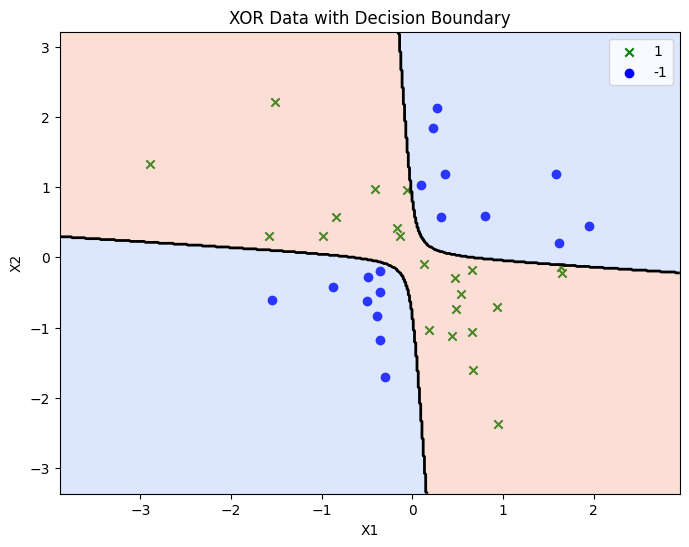
\includegraphics[width=0.6\textwidth]{1.2.c1.png}
  \caption[XOR Data with Decision Boundary]{XOR Data with Decision Boundary}
  \label{1.2.c1}
\end{figure}



The decision boundary in the figure (Regenerative Kernel Hilbert Space) is shown in Figure \ref{1.2.c2}.

\begin{figure}[htbp]
  \centering
  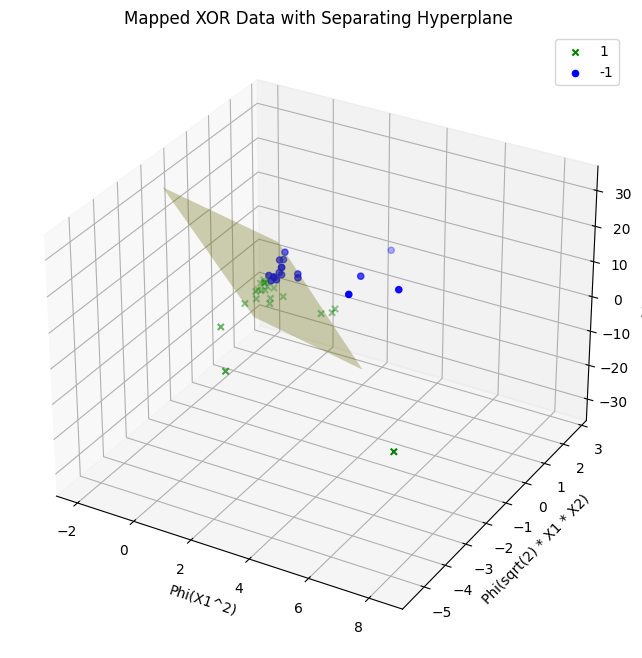
\includegraphics[width=0.6\textwidth]{1.2.c2.png}
  \caption[Mapped XOR Data with Separating Hyperplane]{Mapped XOR Data with Separating Hyperplane}
  \label{1.2.c2}
\end{figure}


\vspace{2mm}
\end{document}
